\documentclass{beamer}

\ifx\narrator\undefined
  \newcommand\narrator{Lisa Simpson}
\fi

\ifx\voice\undefined
  \newcommand\voice{Fiona (mac text2speech)}
\fi

\usepackage[author={narration}]{pdfcomment}
\definestyle{note}{icon=Insert,color=red} 
\newcommand{\pdfnarration}[1]{%
\onslide*<\value{beamerpauses}>{\pdfmargincomment[style=note,author=narration]{#1}}%
}

\newcommand\showpauses{The value of beamerpauses at this point in slide \insertpagenumber\ is: \thebeamerpauses}

\usepackage{amsmath}
\usepackage{tikz, tikz-3dplot, pgfplots} %diagrams
	\usetikzlibrary{calc, hobby, patterns, intersections, angles, quotes, spy, shapes, plotmarks, math, quotes, angles, positioning}

\usepackage{multicol}    %  two columns for problem sections
%\usepackage{picins}      %  to insert small drawings in paragraphs

%Information to be included in the title page:
\title{The Basel Problem}
\subtitle{narrated by \narrator \\
              voiced by \voice \\
              (from Mac Text2Speech)}
\institute{for \\ YouTube}
\date{2021}
\titlegraphic{\includegraphics[width=2cm]{images/Leonhard_Euler.jpeg}}

%\newcommand\pdfnarration[1]{%
%    \pdfmargincomment[style=note,author=narration]{#1} }%

%\pdfnarration{
% [[slnc 2000]]
% In this video we present a modern solution to the Basel problem. 
% [[slnc 2000]]
%}


\begin{document}

\frame{\titlepage}

\begin{frame}
\frametitle{ The Basel Problem }

\alert<1> 
In 1650, Pietro Mengoli, an Italian mathematician, posed, what was later 
called the {\em Basel Problem}: Find the infinite sum of the squares of the recipricols:

\begin{equation*}
  \sum_{n=1}^\infty \frac{1}{n^2} = 1 + \frac{1}{4} + \frac{1}{9} + \frac{1}{16} + \ldots 
\end{equation*}

\pdfnarration{
In 1650, Pietro Mengoli, an Italian mathematician, posed, what was later 
called the {\em Basel Problem}. [[slnc 1000]]
Find the infinite sum of the squares of the recipricols:
}
\pause

\alert<2> 
 In 1734, almost 100 years after it was first posed, the Basel problem was solved by 
a Swiss mathematician, {\em Leonhard Euler}, who showed that
 
\begin{equation*}
  \sum_{n=1}^\infty \frac{1}{n^2} = \frac{\pi}{6}
\end{equation*}

\pdfnarration{
[[slnc 1000]]
 In 1734, almost 100 years after it was first posed, the problem was solved by 
a Swiss mathematician, {\em Leonhard Euler}, 
who showed that the infinite sum of squared reciprocals was exactly Pi by six.
[[slnc 1000]]
}
\pause

\alert<3> 
Here, we present a modern solution to the problem. \\ 
We make use of multivariate calculus to find \\
the value of a certain double integral.

\pdfnarration{
[[slnc 1000]]
Here, we present a modern solution to the Basel problem. 
[[slnc 1000]]
We will make use of multivariate calculus to find the value
of a certain double integral.
[[slnc 1000]]
}

\end{frame}

\begin{frame}
\frametitle{Split the series into even and odd parts \ldots}

\alert<1> 
We set
\begin{equation*}
  S = \sum_{n=1}^\infty \frac{1}{n^2} 
\end{equation*}

then we can split $S$ into even and odd parts
\begin{equation*}
  S = \sum_{n=1}^\infty \frac{1}{(2n)^2}  + \sum_{n=0}^\infty \frac{1}{(2n+1)^2}  = \frac{S}{4}  + \sum_{n=0}^\infty \frac{1}{(2n+1)^2}
\end{equation*}

\pdfnarration{
[[slnc 1000]]
We first split the series into even and odd parts. 
[[slnc 2000]]
Then we note that the even part accounts for one quarter of the total series. 
[[slnc 1000]]
}
\pause

\alert<2> 
which means that
\begin{equation*}
 S =  \frac{4}{3} \sum_{n=0}^\infty \frac{1}{(2n+1)^2}
\end{equation*}

\pdfnarration{
 [[slnc 1000]]
This allows us to express the total series; as four; thirds; of the odd part.
[[slnc 1000]]
}

\end{frame}


\begin{frame}
\frametitle{now express the series as a double integral \ldots}

\alert<1> 
 we have shown
\begin{equation*}
  S  =  \frac{4}{3}  \sum_{n=0}^\infty  \left( \frac{1}{2n+1} \right) \left( \frac{1}{2n+1}\right )
 \end{equation*}
 
 Now we use the fact that any rational number can be expressed as a definite
integral of a power function.
 \begin{equation*}
                   S   =  \frac{4}{3}  \sum_{n=0}^\infty \int_0^1 x^{2n} dx \int_0^1 y^{2n} dy 
 \end{equation*}
 
\pdfnarration{
  [[slnc 1000]]
We use the fact that any rational number; can be expressed as a definite
integral of a [[emph +]] power [[emph -]]  function. 
[[slnc 1000]]
}
\pause

 \alert<2> 
 and collecting terms we have
 \begin{equation*}
                S   =  \frac{4}{3}  \sum_{n=0}^\infty \int_0^1 \int_0^1 (xy)^{2n} dx \; dy
\end{equation*}

\pdfnarration{
 [[slnc 1000]]
Using this trick we change each rational term in the series to an integral. 
[[slnc 1000]]
}


\end{frame}


\begin{frame}
\frametitle{now swap the order \ldots}

\alert<1> 
 swapping the order of summation and integration we have 
\begin{equation*}
    S  =    \frac{4}{3}  \int_0^1 \int_0^1 \left( \sum_{n=0}^\infty (xy)^{2n} \right) dx \; dy
\end{equation*}

\pdfnarration{
 [[slnc 1000]]
Now we swap the order of summation and integration 
[[slnc 1000]]
and we note that the summation inside the integral is
just a [[emph +]] geometric progression [[emph -]].  
[[slnc 1000]]
}
\pause

\alert<2> 
 summing the inner geometric progression we get
\begin{equation*}
      S    =    \frac{4}{3}  \int_0^1 \int_0^1 \left( \frac{1}{1-(xy)^2}  \right) dx \; dy
\end{equation*}

\pdfnarration{
[[slnc 1000]]
 summing the inner  [[emph +]] geometric progression [[emph -]]; using
[[emph +]] elementary [[emph -]] school methods; 
we get this expression for the series
 [[slnc 1000]]
}
\pause

\alert<3>
so now we need only evaluate this double integral over the unit square which we
will do after refreshing our knowledge of change of variable formula for double integrals.

\pdfnarration{
[[slnc 1000]]
Now we need only evaluate a double [[emph +]] integral [[emph -]] over the unit square
[[slnc 1000]]
We will perform this integration using a change of variable technique which we outline 
on the next slide.
[[slnc 1000]]
}

\end{frame}

\begin{frame}
\frametitle{change of variables for double integrals \ldots}

The change of variable formula for a double integral goes like this:

\begin{equation*}
     \iint_R f(x,y) dx \; dy = \iint_T f(x(u,v),y(u,v)) \left| \frac{\partial( x, y)}{\partial(u,v))} \right| du \; dv
\end{equation*}

where the transformation $(u,v) \rightarrow \left( x(u,v),y(u,v) \right)$ is a {\em one-to-one} differentiable map from $T$ onto $R$ 
with Jacobian:
     
\begin{equation*}
     J = \left| \frac{\partial( x, y)}{\partial(u,v))} \right| = 
     \left|
        \begin{array}{cc}
             \frac{\partial x}{\partial u}  & \frac{\partial x}{\partial v}   \vspace{3pt} \\
             \frac{\partial y}{\partial u}  & \frac{\partial y}{\partial v}
         \end{array} \right|
\end{equation*}     

\pdfnarration{
 [[slnc 2000]]
This is the change of variable formula for a double integral over a region; R.
 [[slnc 2000]]
We transform from one coordinate system to another using a one to one; smooth; and invertible; mapping.
  [[slnc 2000]]
}


\end{frame}

\begin{frame}
\frametitle{Back to our problem \ldots}

\alert<1>
To evaluate our double integral, the substitution we will attempt is
\begin{equation*}
     x(u,v) = \frac{\sin u}{\cos v}  \text{ \; and \; }  y(u,v) = \frac{\sin v}{\cos u} 
\end{equation*}
\pdfnarration{
 [[slnc 1000]]
To evaluate [[emph +]] our [[emph -]] double integral we transform the coordinates;
using reciprocals of sinusoidals.  
[[slnc 2000]]
}
\pause

\alert<2>
with Jacobian 
\begin{eqnarray*}
     J = \left[ 
        \begin{array}{cc}
             \frac{\partial x}{\partial u}  & \frac{\partial x}{\partial v}   \vspace{3pt} \\
             \frac{\partial y}{\partial u}  & \frac{\partial y}{\partial v}
         \end{array} \right]  
         = \left[ 
        \begin{array}{cc}
             \frac{\cos u}{\cos v}  & - \frac{\sin u \sin v}{\cos^2 v}   \vspace{3pt} \\
             - \frac{\sin v \sin u}{\cos^2 u}  & \frac{\cos v}{\cos u}
         \end{array} \right] 
\end{eqnarray*}

who's determinant evaluates to
\begin{equation*}
     |J|  =  1 -  \left(\frac{ \sin u \sin v }{\cos v \cos u}\right)^2 = 1 - (xy)^2 
\end{equation*}
\pdfnarration{ 
[[slnc 1000]]
The determinant of the Jacobian simplifies considerably. 
 [[slnc 2000]]
 }
 \pause
 
 \alert<3>
Our double integral for the sum of the series transforms as follows
\begin{align*}
      S   &=    \frac{4}{3}  \iint_{I \times I} \left( \frac{1}{1-(xy)^2}  \right) dx \; dy \\
           &=  \frac{4}{3}  \iint_{T} \left( 1 \right) du \; dv = \frac{4}{3} \text{Area}(T)
\end{align*}

\pdfnarration{ 
[[slnc 2000]]
and the double integral simplifies as well. 
[[slnc 2000]]
We end up integrating the unit function over a region; T; still to be determined. 
 [[slnc 2000]]
 }

     
\end{frame}

\begin{frame}
\frametitle{Finding $T$ \ldots}

\alert<1>
It remains to find a region $T$ in the $u \; v$ coordinate system that maps to the 
unit square under the transformation:
\begin{equation*}
     x(u,v) = \frac{\sin u}{\cos v}  \text{ \; and \; }  y(u,v) = \frac{\sin v}{\cos u} 
\end{equation*}
\pdfnarration{
 [[slnc 1000]]
It remains to find a region $T$ in the new coordinate system that maps to the 
unit square in the old coordinate system under our transformation.
[[slnc 2000]]
}
\pause

\alert<2>
Consider the inequalities that define the unit square:
\begin{equation*}
      0   \leq  x  \leq 1\text{ \; and \; } 0 \leq y \leq 1
\end{equation*}
transforming to $u \; v$ coordinates and multiplying through by the cosine terms we require:
\begin{equation*}
      0   \leq  \sin u  \leq \cos v \text{ \; and \; } 0 \leq  \sin v \leq \cos u
\end{equation*}
\pdfnarration{
 [[slnc 1000]]
We use our transformation to produce inequalities for the region T in the u v plane.
[[slnc 2000]]
}

\end{frame}


\begin{frame}
\frametitle{Sketching $T$ \ldots}

\alert<1>
The region $T$ must satisfy:
\begin{equation*}
      0   \leq  \sin u  \leq \cos v \text{ \; and \; } 0 \leq  \sin v \leq \cos u
\end{equation*}
The left inequalities are satisfied if both $u$ and $v$ are greater than $0$

whilst the right hand inequalities are satisfied if 
\begin{equation*}
 \sin u \leq \sin(\frac{\pi}{2} - v) \text{ \; and \; } \sin v \leq \sin(\frac{\pi}{2}-u) 
 \end{equation*}
 
Both of these are satisfied if $ u + v \leq \frac{\pi}{2}$.
\pdfnarration{
 [[slnc 1000]]
The left hand inequalities are satisfied if both u and v are greater than zero.
[[slnc 1000]]
Whilst the right hand inequalities are satisfied if u plus v is less than pi by two.
[[slnc 2000]]
}

\pause

\alert<2>

\begin{multicols}{3}
  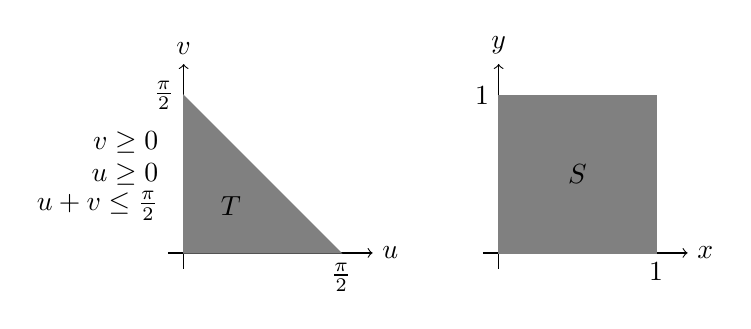
\begin{tikzpicture}[scale=2,
          domain=-1:1,
          declare function = {f(\x) = exp(\x);
         }]
          
  \draw[->] (-0.1,0)--(1.2,0) node[right]{$u$};
  \draw[->] (0,-0.1)--(0,1.2) node[above]{$v$};  
  \draw (-0.1, 0.7) node[left] {$v \geq 0$};
  \draw (-0.1, 0.5) node[left]{$u \geq 0$};
  \draw (-0.1, 0.3) node[left]{$u  + v \leq \frac{\pi}{2}$};
  \draw (1,0) node[below]{$\frac{\pi}{2}$};
  \draw (0,1) node[left]{$\frac{\pi}{2}$};
  \filldraw[gray] (0,0)--(1,0)--(0,1)--cycle;
    \draw[color=black] (0.3,0.3) node{$T$};
    
     \draw[->] (1.9,0)--(3.2,0) node[right]{$x$};
  \draw[->] (2,-0.1)--(2,1.2) node[above]{$y$};  
  \draw (3,0) node[below]{$1$};
  \draw (2,1) node[left]{$1$};
  \filldraw[gray] (2,0)--(3,0)--(3,1)--(2,1)--cycle;
    \draw[color=black] (2.5,0.5) node{$S$};

 \end{tikzpicture}
  
\end{multicols}

\pdfnarration{
 [[slnc 1000]]
We now have all the information we need to sketch the region, T, which maps
to the unit square, S, under our change of variable transformation.
[[slnc 2000]]
}

\end{frame}

\begin{frame}
\frametitle{Wrapping it up \ldots}

\alert<1>
We have shown that $T$ is a triangle in the positive quadrant of the
$u \; v$ plane with base and height of size $\frac{\pi}{2}$. 
\pdfnarration{ 
[[slnc 2000]]
We have shown that T; is a triangle in the positive quadrant;
with base and height of size pi by two 
 [[slnc 2000]]
 }
\pause

\alert<2>
We can now calculate the sum of our series:
\begin{align*}
      S &=  \frac{4}{3} \iint_T \left( 1 \right) du \; dv \\
          &=   \frac{4}{3} \text{Area}(T) \\
          &= \frac{4}{3} \left( \frac{\pi}{8} \right) \\
          &= \frac{\pi}{6}
\end{align*}
\pdfnarration{ 
[[slnc 2000]]
The area of T is half base times height; and thus pi by eight.
[[slnc 1000]]
The sum of our series is four thirds of the area.
 [[slnc 1000]]
 So the infinite sum of the recipricols is pi by six; and we are done.
 [[slnc 2000]]
 }

\end{frame}

\begin{frame}
\frametitle{Bibliography}

\begin{thebibliography}{99}

\bibitem{JoeBreen} Joe Breen Math, Youtube video, {\em The Basel problem}, \url{https://www.youtube.com/watch?v=MB2HBH_ykf0}

\end{thebibliography}
\pdfnarration{
[[slnc 2000]]
We would like to acknowledge the resources shown here as they were most helpful in the compilation of these slides.
[[slnc 1000]]
}

\end{frame}


\end{document}
